% 修士論文テンプレート

\documentclass[10pt]{jreport}

\usepackage{master_thesis}
\usepackage{./grad}
\usepackage[dvipdfmx]{graphicx}
\usepackage{here}
\usepackage{url}
\usepackage{bm}
\usepackage{comment}
\usepackage{cite}
\usepackage{amsmath,amssymb,amsfonts}
\usepackage{algorithmic}
\usepackage{graphicx}
\usepackage{textcomp}
\usepackage{xcolor}

% A4 : width 21cm, height 29.7cm
\usepackage[a4paper,textheight=21.7cm,top=3cm,left=2cm,right=2cm,headheight=15pt]{geometry}

\年度{2021}
\題目{VANETにおける車両位置とリンク状態を考慮した地理的
opportunistic routing}
\指導教官{野口 拓}
\学籍番号{6611200033-0}
\氏名{高橋 柊人}
\コース{計算機科学コース} %計算機科学コース or 人間情報科学コース


\begin{document}
% 表紙 %%%
\maketitle


\renewcommand{\thepage}{\roman{page}}
\setcounter{page}{1}
\addcontentsline{toc}{chapter}{内容梗概}
\chapter*{内容梗概}
本論文は,筆者が立命館大学情報理工学研究科において行った「VANETにおける車両位置とリンク状態を考慮した地理的
opportunistic routing」の成果をまとめたものである.

test


\newpage
\pagestyle{myheadings}
\renewcommand{\thepage}{\roman{page}}
%\setcounter{page}{1}
\addcontentsline{toc}{chapter}{目次}
%\setcounter{page}{1}
\tableofcontents


\newpage
\renewcommand{\thepage}{\arabic{page}}
\setcounter{page}{1}
\chapter{緒論}
\vspace{-5mm}

高速道路や一般道での無謀な運転や不注意運転によるほかのドライバへの危険が問題となっている. もし, これらの危険行為を行う車両の接近を遭遇する以前に知ることができれば, 多くの事故を減らすことができる可能性がある. 交通死亡事故の原因の中では, 規制速度を超過した場合の割合が31.6%\cite{1}と, 速度違反が死亡事故につながることがわかる. また, 交通事故死亡者数と取り締まり件数に注目すると, 取り締まりが増加すると死者数が減少するデータもある. これらのことから, 交通事故の死亡者数を減らすためには, より多くの速度超過の監視が求められる. 
 

そこで本論文では, VANETを用いたブロードキャスト数を最小限に抑えたVANETを用いた速度超過車両検出手法を提案する.速度超過車両の検出確率や,ブロードキャスト数を調査し,有効性を示す.

第2章では, VANETの概要を説明し, 既存方式について述べる. 第3章では, VANETを用いた速度推定法, ネットワークトラヒック量の削減を目的としたブロードキャスト制御アルゴリズムについて述べる. 第4章では, 評価方法について述べ, 本研究の評価方法を基に検証した結果をまとめる. 第5章は結論であり, 本研究の主な結果をまとめる. 



\chapter{VANET}
\vspace{-5mm}
\section{概要}
近年, 情報通信技術の発達により, 無線通信を用いて車両間または, 路車間で情報をやり取りすることによって交通事故や渋滞などの道路交通問題の解決を目指す高度道路交通システム(ITS:Inteligent Transport System)が注目を浴びている\cite{sample7}. ITSの代表的なサービスとして, 渋滞情報と連動した高度なナビゲーションシステム(VICS::Vehicle Information and Communication System)\cite{sample8}や, 自動料金収受システム(ETC:Electronic Toll Collection)\cite{sample9}などがあげられる. これらのサービスを支える技術として, 路車間通信と車両アドホックネットワーク(VANET)がある. 路車間通信は車両が路側機のインフラ設備との無線通信により情報のやりとりを行う. しかし, 路車間通信はインフラ設備の設置にかかる費用と, 設置場所が限定される可能性があるという問題が存在する. 一方, VANETは車両同士で通信を行うためインフラ設備の整備されていない不特定の場所でも通信を行うことが可能になる. VANETのアプリケーションとして, 渋滞回避情報の伝搬, 緊急車両情報の警告など, 安全運転支援に期待されている. 
\section{車車間通信}
車車間通信は車両と車両との間で無線通信を行い, 情報のやり取りを行うものである. 車車間通信を図2.1に示す. 車車間通信では, 端末同士(車両同士)で自律的にネットワークを構築し, 宛先に直接通信できない場合には間の車両が中継車両となり, マルチホップ通信を行う. 車車間通信のメリットは固定のインフラを必要とせず車両間のみで通信が可能になり, インフラが存在しない地点で通信が可能になることである. 
\section{路車間通信}
路車間通信は, 道路に設置された路側機(RSU:Road Side Unit)と車両で無線通信を行い 
様々な情報の交換を行うものである. 路車間通信を図\ref{fig:VANET}に示す.  路車間通信の代表的なサービスとしてVICS(Vehicle Information and Communication System)やETC(Electronic Toll Collection)がある. VICSは, 各道路に設置されたビーコンから道路交通情報を発信し, 車載のカーナビや高速道路の電子掲示板に高速道路の渋滞の情報, 区間を通過するための所要時間, 駐車場情報などを表示する「ナビゲーションシステム高度化」を目指したサービスである. ETCは高速道路の入り口に設置されている通信機と車載の通信機で無線通信を行い, 料金所に止まることなく, 自動でスムーズに料金の支払いができるシステムである. 料金所での一時停止が渋滞の原因の一つであったが, ETCの導入で渋滞を解消することができた. 




%図の入れ方
\begin{figure}[!ht]
\centering
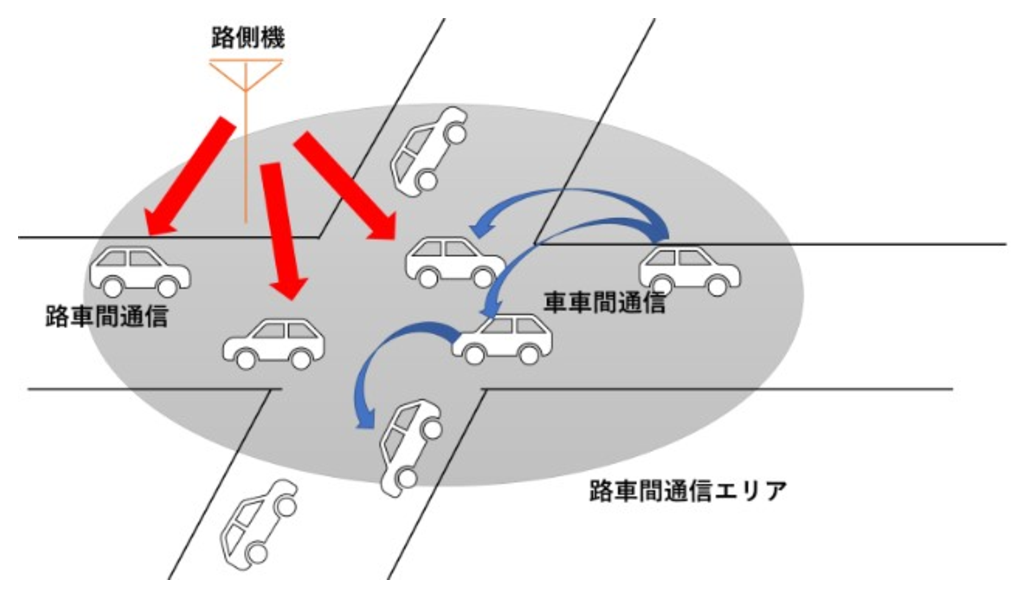
\includegraphics[width=15cm]{figures/VANET.eps}
\caption{車車間通信と路車間通信}
\label{fig:VANET}
\end{figure}


\section{ルーチングプロトコル}
\label{RoutingProtocol}
VANETを都市環境で展開する場合, 高速な移動性, 不均一な車両密度, 樹木や建物による電波の遮断など様々な要件を考慮する必要がある. この様々な要件に対応するため, 多種多様なルーチングプロトコルが提案されている\cite{2}. 次節以降でそれぞれのルーチングプロトコルの特徴について述べる.

\subsection{Topology-based routing}
\label{Topology}
Topology-base routing\cite {3,4,5} は, ネットワークに存在するリンクに関する情報を使用して, パケット転送を行う方式である. Topology-based routingはProactive型とReactive型に分類できる. 前者は, ノード間で周期的な制御パケットの交換を行うことにより, 各ノードがすべての宛先ノードへの経路情報を常時保持する方式である. 後者は, 最初は経路情報は保持しておらず, 通信要求が生じてから, 制御パケットを交換し経路情報を作成する方式である. 前者と比較して後者は, 制御パケットのオーバヘッドを抑えられるというメリットがある. 
しかし, これらのTopology-based routingは, ノードが頻繁に移動するVANETにおいては, 経路情報を定期的に変更する必要がある.
したがって, 制御パケットのオーバーヘッドが増加するためVANETには適していない.

\subsection{Geographic routing}
\label{Geographic}
Geographic routing\cite{6,7,8,9,10,11,12,13,14,15} は, 隣接ノードの位置情報と宛先ノードの位置に基づいてパケット転送を行う方式である. このタイプのルーチングプロトコルは, Topology-based routingのように確立されたルートを維持する必要がない. したがってGeographic routingは制御パケットを使用する必要がないため, 少ないパケット数でトポロジーの変化に対応することができる. Greedy fowardingはGeographic routingにおいて有名な方式の一つである. Greedy fowardingは隣接ノードの中で最も宛先ノードに近いノードを中継ノードとして選択することで, ホップ数やオーバヘッドの削減を示している. しかし, 実際の都市環境では, 建物によるシャドウイングや距離による電波強度の低下によりパケットのドロップ率が高くなる可能性がある. 

\subsection{Opportunistic routing}
\label{Opportunistic}
上記のルーチングの問題点を解決できる可能性がある, Opportunistic routing\cite{16} が近年注目を集めている. Opportunistic routingと前述したルーチングプロトコルとの主な違いは固定経路を使用せず, 送信ノードが次の中継ノードを1つに決定しないことである(図\ref{fig:Gegraphic_opportunistic}). Opportunistic routingではブロードキャストの性質を利用し, 受信したノード同士が協調しパケットを再ブロードキャストするか否かを決定することでパケット到達率の向上とオーバーヘッドの削減を果たしている. 

Opportunistic routingは主に次の4ステップで構成されている.

\begin{itemize}
	\item 中継候補ノードセット(RCS) の選択
	\item RCSの優先順位を決定
	\item RCSへのブロードキャスト
	\item 優先順位に応じた再ブロードキャストをするか否かの決定(RCS同士の協調)
\end{itemize}

図\ref{fig:Basic1}, \ref{fig:Basic2}にOpportunistic routingの基本モデルを示す.
$N_{s}$が送信ノード, $N_{d}$が宛先ノードである. 送信ノード$N_{s}$はRCSとして$N_{1}$ ~ $N_{n}$を選択する. 次に送信ノードは選択したRCSそれぞれに優先順位を指定してパケットをブロードキャストする. 受信した$N_{1}$ ~ $N_{n}$のノードはそれぞれ自身の優先順位を確認し, 中継タイマー(待ち時間)を設定する. 中継タイマーは優先順位が高いノードほど早くタイムアウトするように設定し, タイマーが切れたノードから再ブロードキャストを行う. 自身の中継タイマーが切れる前に自身より優先順位が高いノードの再ブロードキャストを受信した場合, 自身の再ブロードキャストをキャンセルし, 冗長なパケットの増加を防ぐ.
 

\begin{figure}[!ht]
	\centering
	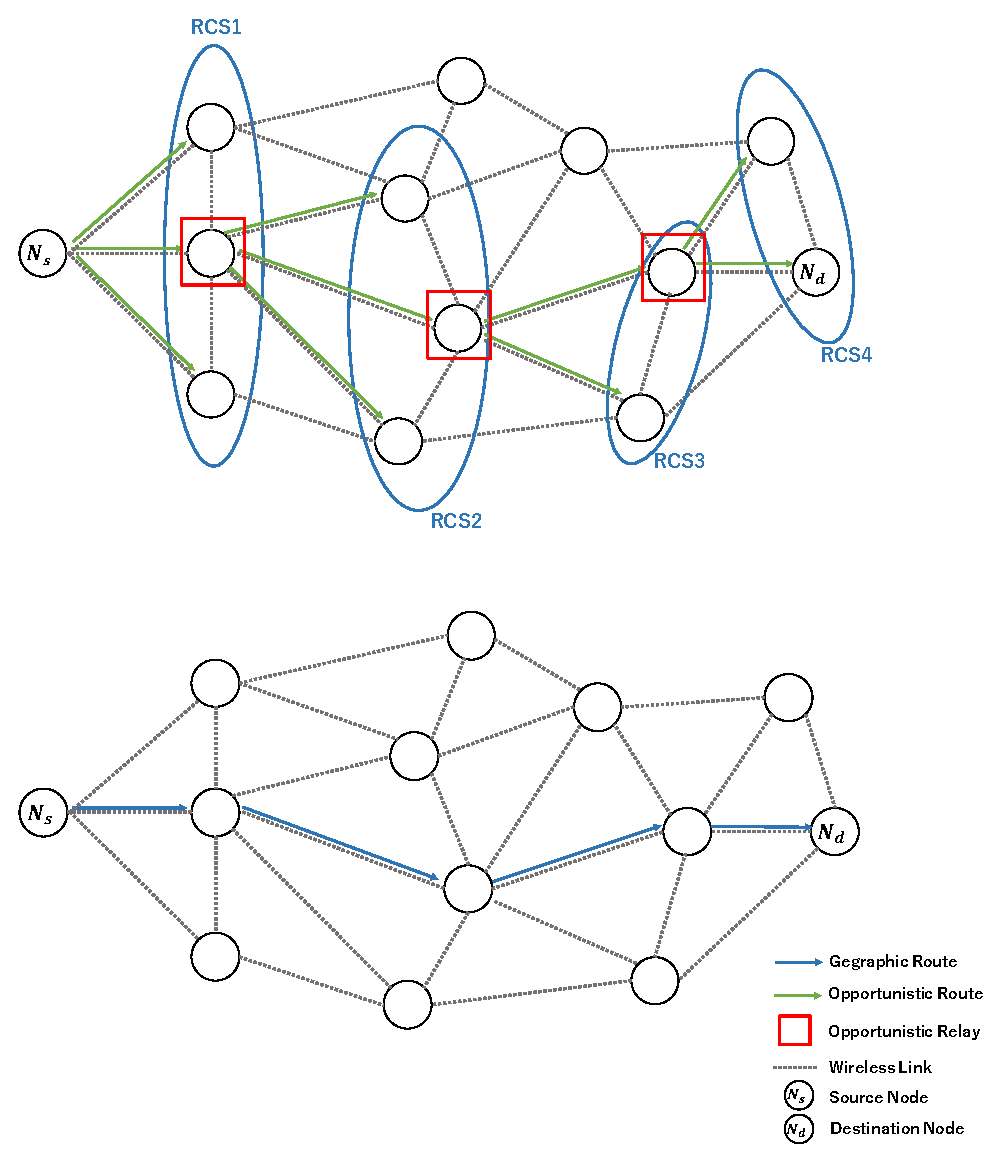
\includegraphics[width=150mm]{figures/difference_geographic_opportunistic.eps}
	\caption{Geographic routingとOpportunistic routing}
	\label{fig:Gegraphic_opportunistic}
\end{figure}

\begin{figure}[!ht]
	\centering
	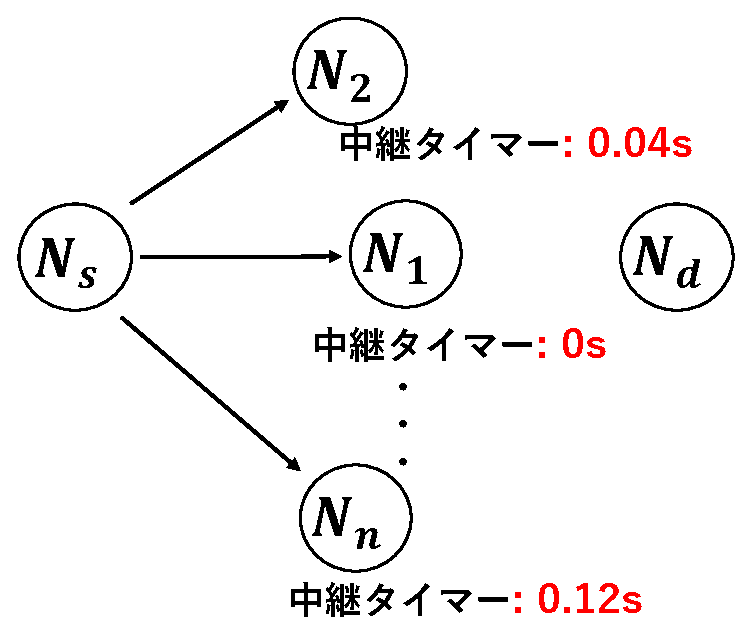
\includegraphics[width=90mm]{figures/basic-opportunity1.eps}
	\caption{Opportunistic routingの基本モデル1}
	\label{fig:Basic1}
\end{figure}

\begin{figure}[!ht]
	\centering
	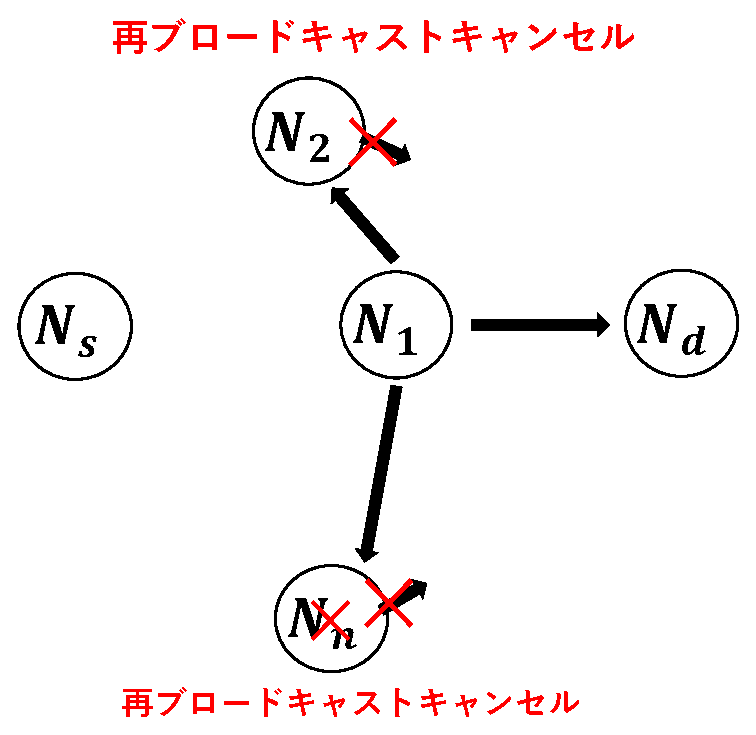
\includegraphics[width=90mm]{figures/basic-opportunity2.eps}
	\caption{Opportunistic routingの基本モデル2}
	\label{fig:Basic2}
\end{figure}

これらのことから, Opportunistic routingにおいて, 優先順位決定アルゴリズムが通信性能に直接影響を及ぼすことがわかる.

代表的なOpportunistic routingとしてOpportunistic multi-hop routing fo wireless networks(EXOR) \cite{16}が提案されている. これは, RCSの優先順位を決定するメトリックとして, Expected transmission cost(ETX) \cite{21}を用いている. しかし, ETX値はVANETの性質であるノードのランダムで高速なモビリティを考慮していないという問題がある.

そこで, 新たにVANETに適したETX値を考案したLink state aware geographic opportunistic routing protocol(LSGO) \cite{18}が提案された. LSGOでは, VANET用に最適化されたETX値をRCSの優先順位を決定するメトリックとして使用し, パケット到達率の向上, エンドツーエンド遅延の減少を実現している. また, Collision-aware opportunistic routing protocol (SCAOR) \cite{22}では, パケットの衝突でネットワークパフォーマンスを低下させる問題を防ぐために, ノード密度パラメータをRCSの優先順位を決定するメトリックとして追加した. その結果, 高速道路においてEXORやLSGOに比べ通信性能が向上することを示している. Hybrid opportunistic and position-based routing  protocol (OPBR) \cite{23}では, パケットがRCSに到達しない場合, 遅延が増加するという問題を解決するために, 隣接ノードの位置情報からリンクの切断を推測した. この結果パケット到達率の向上, エンドツーエンド遅延の減少を示している.

しかし, 既存のopportunistic routingの多くは, 都市環境を想定して考案されているが, 性能評価で建物によるシャドウイングの影響が考慮されておらず, 通信性能を過大評価している可能性がある. また, これによりシャドウイングの影響を考慮したルーティングプロトコルが設計されていない可能性がある. 

そこで, 本研究では, 既存opportunistic routingであるLSGOをネットワークシミュレータNS-3\cite{19}のシャドウイングモデルであるObstacle Shadowing Model\cite{20}を用いて評価し, 建物によるシャドウイングが起こる場合と起こらない場合の通信性能を検証し, 問題点を明らかにする.


\subsection{Geocast routing}
これまでの節では, ある特定ノードにデータを届けるUnicast routing protocolを紹介した.
本節では, ある特定領域にいる全ノードにデータを届けるGeocast routing protocol\cite{Geocast}について紹介する.
特定領域にいる多くのノードに情報を届けるために, 最も単純な方式がフラッディング手法である.
しかし, フラッディング手法はパケットを受信したすべてのノードがブロードキャストをするため, ブロードキャストストームの発生する確率が高まる.
そこで, 宛先方向へのフラッディングを行う指向性フラッディングがある. 指向性フラッディングの代表例として, Location-Based-Multicast (LBM) \cite{LBM}が提案されている.
LBMでは, 宛先領域(Geocast Region)と転送エリアを表す(Forwarding Region)を用いるLBM scheme1, データパケットを受け取ったノードが, 自身と宛先領域の中心座標との距離を算出し, 自身が送信ノードより宛先領域の中心座標に近い倍のみデータパケットを転送するLBM scheme2の2種類の転送手法が手案されている.
scheme1, scheme2の動作例を図\ref{fig:scheme1}, \ref{fig:scheme2}に示す.

\par
\vspace{5mm}
\noindent
\textbf{LBM Scheme1}
\vspace{5mm}

Scheme1の手順を以下の(1)~(4)に示す.


\textbf{手順 1} ソースノード$S$は, 矩形領域$OPQB$をGeocast regionとして指定する.

\textbf{手順 2} $S$は, 自身とGeocast regionを含む最小の矩形$ASCB$をForwarding Regionとして指定する. その後, Forwarding Regionの情報を含めたデータパケットをフラッディングする.

\textbf{手順 3} データパケットを受信したノードは,自身がForwarding Region内にいる場合,自身とGeocast Regionを含むForwarding Regionを再設定しフラッディングを行う.自身がForwarding Region外にいる場合,データパケットを破棄する.

\textbf{手順 4} Geocast Regionに到達するまで手順3を繰り返す. 


\begin{figure}[!ht]
	\centering
	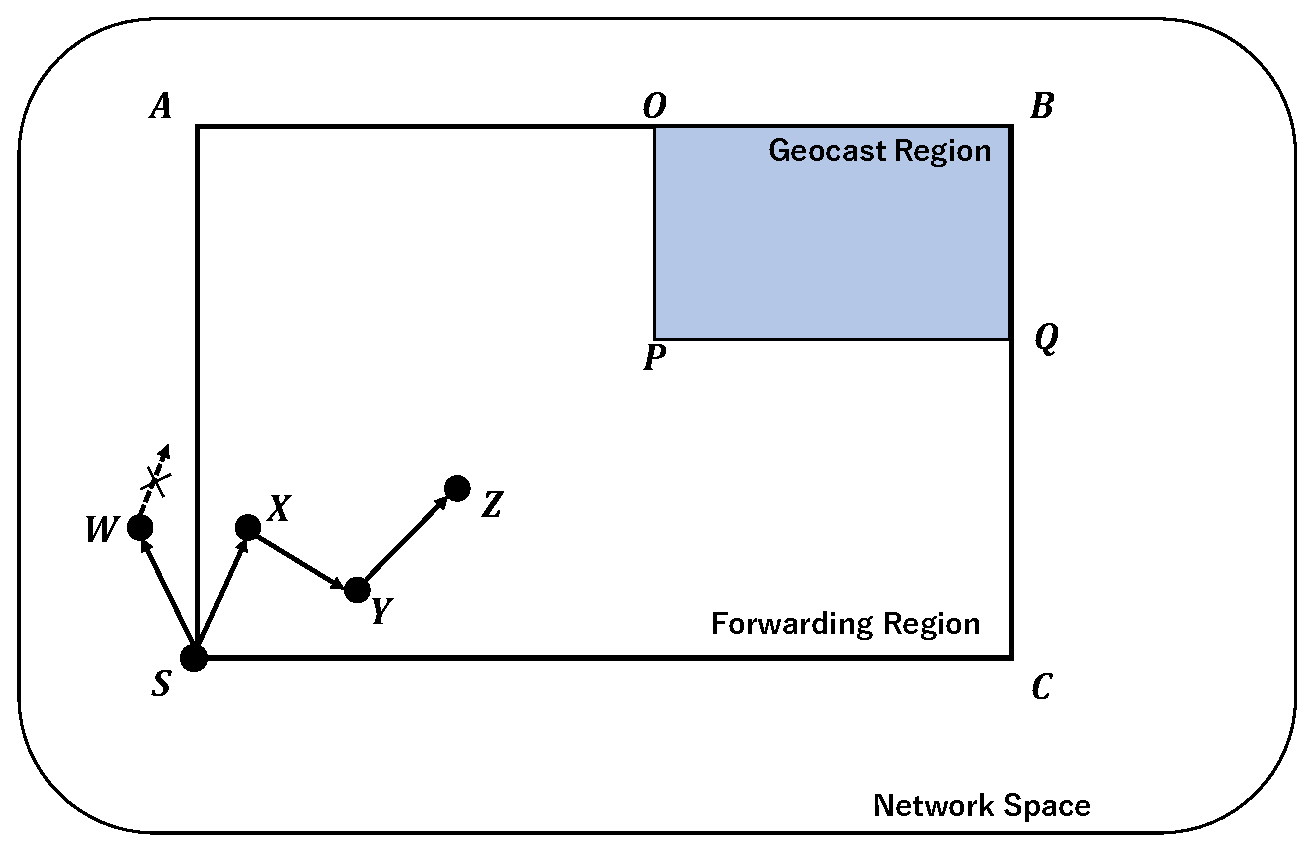
\includegraphics[width=100mm]{figures/Scheme1.eps}
	\caption{LBM:scheme1}
	\label{fig:scheme1}
\end{figure}

\par
\vspace{5mm}
\noindent
\textbf{LBM Scheme1}
\vspace{5mm}

Scheme2の手順を以下の(1)~(3)に示す.


\textbf{手順 1} ソースノード$S$は, Multicast Regionの中心座標と自身の位置情報を含めたデータパケットをフラッディングする.

\textbf{手順 2} データパケットを受信した各ノードは, 1ホップ前のノード(ノード$X$の場合のノード$S$)の位置情報と, 自身の位置情報を確認し, それぞれのMulticast regionの中心座標までの距離($Dist$)を算出する. 1ホップ前のノードより自身がMulticast regionの中心座標に近い場合, データパケットに自身の位置情報を再設定しフラッディングを行う.
例えば, 図の場合$Dist_x$ \verb|<| $Dist_x$の関係が成り立つため, ノード$X$はノード$S$からパケットを受信した場合, フラッディングを行う. しかし, $Dist_x$ \verb|<| $Dist_y$の関係が成り立つ, ノード$X$からのパケットをノード$Y$が受信した場合, データパケットを破棄する.

\textbf{手順 3} Geocast Regionに到達するまで手順2を繰り返す.



\begin{figure}[!ht]
	\centering
	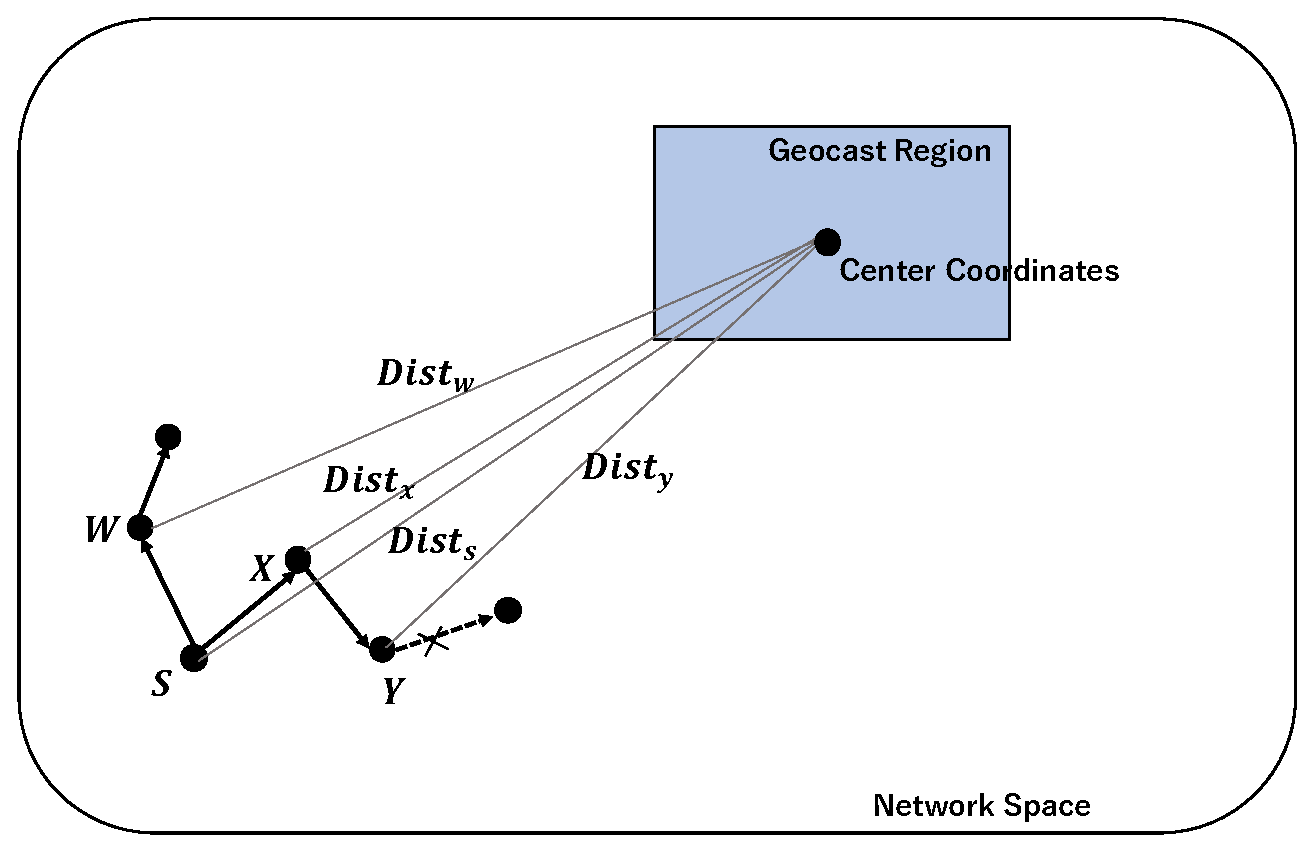
\includegraphics[width=100mm]{figures/Scheme2.eps}
	\caption{LBM:scheme2}
	\label{fig:scheme2}
\end{figure}

本研究では, 提案するOpportunistic routingを拡張し, Geocast routingにおいても有効であることを示す.



\section{Local optimum problem}
\label{local_optimum_problem}
\ref{Geographic}節で紹介したGeographic routingの既存研究では, 各送信ノードは自分より宛先ノードに近い隣接ノードの中から中継ノードとして最適なノードを1つ選択する. 同様に\ref{Opportunistic}節で紹介した多くのVANET用に設計されたOpportunistic routingにおいても, 各送信ノードは自分より宛先ノードに近い隣接ノードの中からCRSを選択する. しかし, 時には自分より宛先ノードに近い隣接ノードが存在しない場合が発生する. この問題をLocal optimum problem\cite{6}と呼ぶ. Local optimum problemは, 図\ref{fig:Local_optimum}のように建物による電波の遮断が起きやすい都市環境では発生確率が上昇する. したがって, 特にVANETにおいて自分より宛先ノードに近い隣接ノードから中継ノードを選択するタイプのルーティングでは, この問題を防ぐアプローチと発生した場合の対処法(recovery strategy) の考案が必用である.

\begin{figure}[!ht]
	\centering
	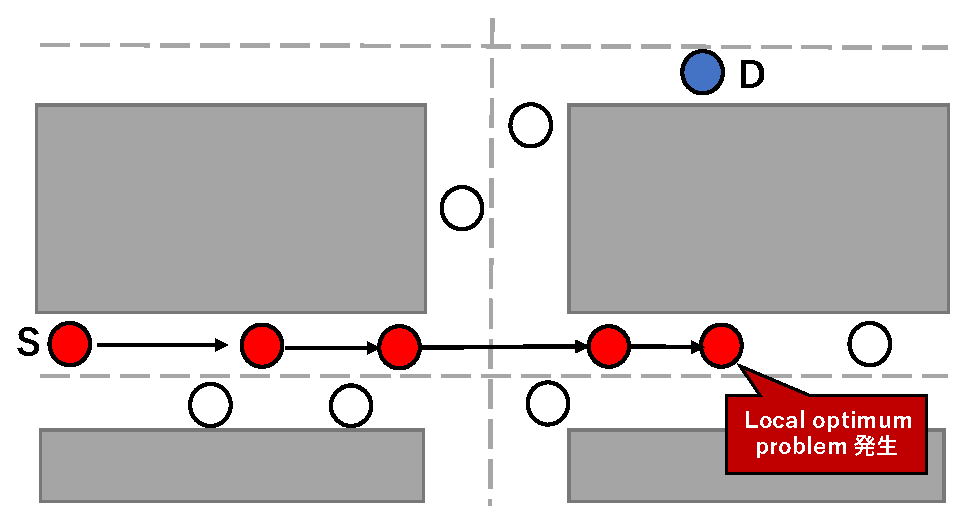
\includegraphics[width=130mm]{figures/Local_optimum_problem.eps}
	\caption{Local optimum problem}
	\label{fig:Local_optimum}
\end{figure}

\section{Recovery strategy}
前節で説明したLocal optimum problemがルーチング中に発生した場合, これに対処する中継戦略が必要となる. これをRecovery strategy\cite{28}と呼ぶ. revovery strategyの基本モデルを図\ref{fig:Recovery}に示す. $N_{1}$でLocal optimum problemが発生する. 次に$N_{1}$は, 自身の位置情報をパケットに加えrecovery strategyを開始する. recovery strategyは, Local optimum problemが発生したノード($N_{1}$)の位置より宛先に近いノードにパケットが到達するまで繰り返される. $N_{2}$までパケットが到達した場合$N_{2}$は$N_{1}$よりも宛先に近いため, 元の中継を開始する. 
  

\begin{figure}[!ht]
	\centering
	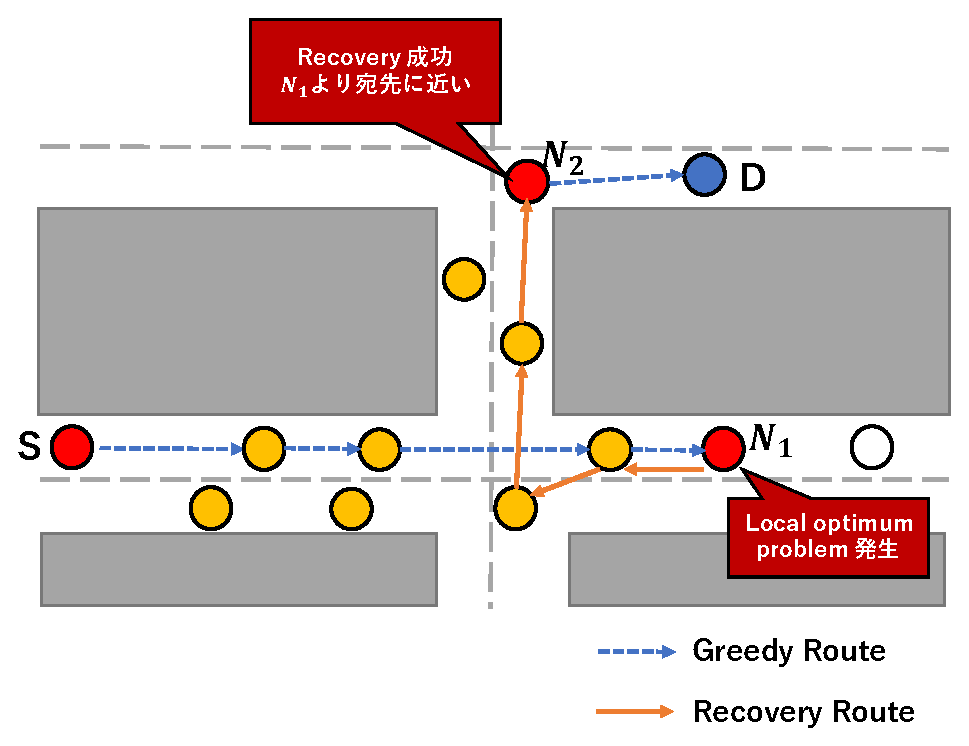
\includegraphics[width=130mm]{figures/basic-recovery.eps}
	\caption{Recovery strategy}
	\label{fig:Recovery}
\end{figure}

代表的なrecovery strategyとしてGreedy perimeter stateless routing(GPSR) \cite{6}の perimeter forwarding
と呼ばれるrecovery strategyが提案されている. perimeter forwardingの例を図\ref{fig:Perimeter}に示す. perimeter fowardingではグラフ理論で古くからよく知られている右手の法則を使用する. この図では送信ノード$S$が宛先ノード$D$に最も近いためLocal optimum problemが発生している. この場合, 送信ノードは自分と宛先ノードを結んだ線から反時計回りに隣接ノードを探索し, 最初に発見したノードに対してパケットを送信する. perimeter forwardingの2ホップ目以降では, 1ホップ前のノード(ノードxの場合はノードS)と自ノードを直線で結び, この直線から半時計回りに探索したノードに対してパケットを送信する. これを繰り返すことにより迂回ルートを構築することが可能になる. 
しかし, 右手の法則を使用する場合, すべてのエッジが交差していない必要がある. 例えば図\ref{fig:cross_link}のようなエッジ(リンク) の接続状態の場合(x → u → z → w → u → x)のようにループが発生する可能性がある. GPSRではループの原因となるクロスリンクを削除する方式が提案されているが, この方式は障害物が多く存在する都市環境ではネットワークの切断につながる可能性がある. したがって, perimeter fowardingはVANETには適していない.




\begin{figure}[!ht]
	\centering
	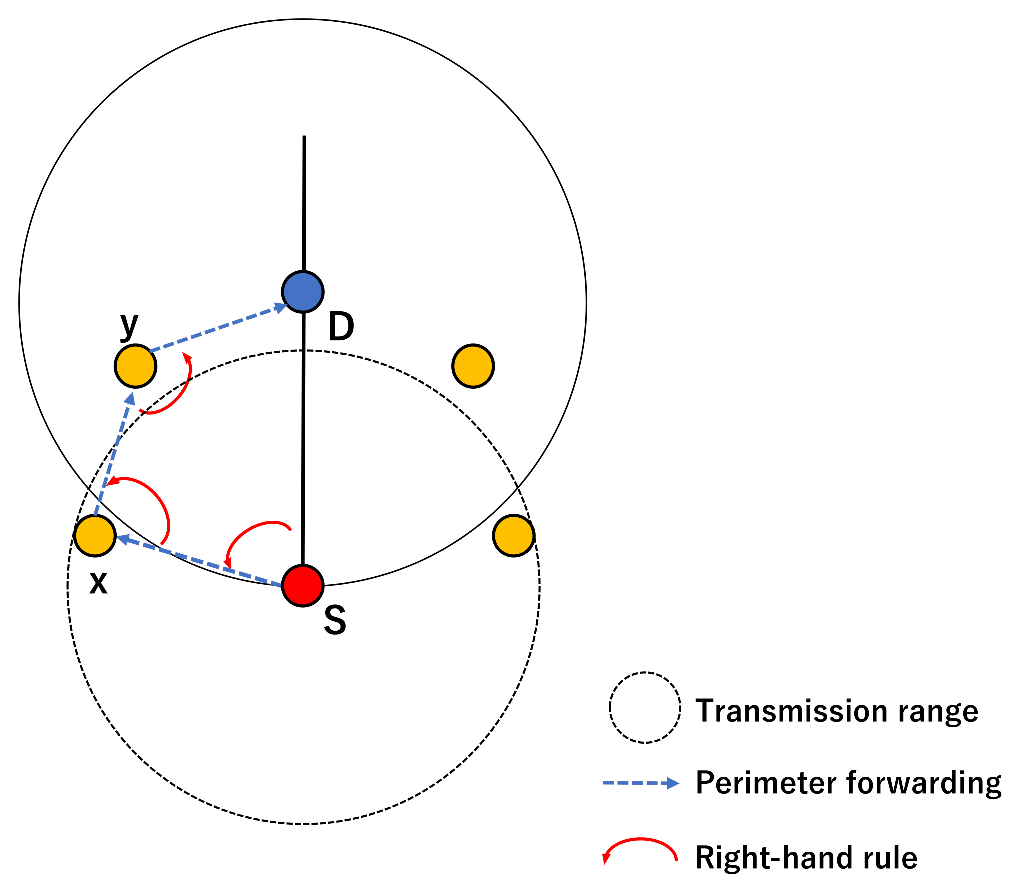
\includegraphics[width=130mm]{figures/Perimeter.eps}
	\caption{Perimeter fowarding}
	\label{fig:Perimeter}
\end{figure}

\begin{figure}[!ht]
	\centering
	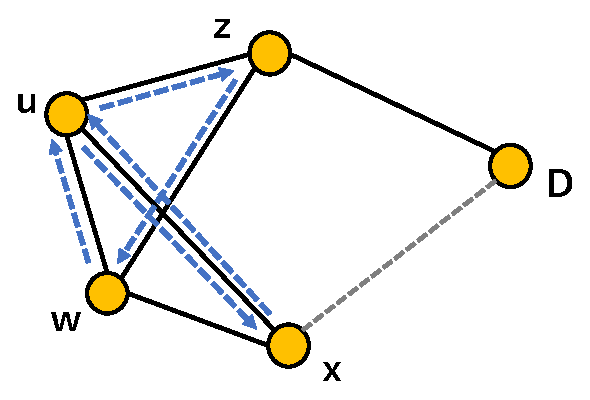
\includegraphics[width=100mm]{figures/cross-link.eps}
	\caption{ループが発生する例}
	\label{fig:cross_link}
\end{figure}

GPSRの問題点に対処するため, Greedy Perimeter Coordinator Routing(GPCR)\cite{7}が都市環境用に提案された. GPCRのrecovery strategyにおける主なアイデアは, Coordinatorと呼ばれる交差点に位置するノードを中継ノードとして最も優先して選択することである. GPCRのrecovery strategyの例を図\ref{fig:GPCR}に示す.
GPCRのrecovery strategyは, 右手の法則を使用した道路の選択と同一道路内の制限されたgreedy fowardingの2つの手順を繰り返し行う. 図ではLocal optimum problemが発生したノード$S$が転送する道路を選択し, 次の交差点を目指しgreedy fowardingを行う. パケットが交差点ノード$C_{1}$に到達すると, $C_{1}$は右手の法則を使用し, 転送する道路を選択する. この手順を繰り返す. GPCRでは, 各交差点にノードが存在する場合, GPSRのようにクロスリンクによるループは発生しない. しかし, 交差点ノードが存在しない場合ループが発生するという問題が生じる. この問題を解決するため, VANET cross Link Corrected Routing (VCLCR) \cite{29} が提案されている. VCLCRでは, 転送中の道路IDをパケットに格納することで, ルーチングループを検知し, クロスリンクを削除する. しかし, この方式ではパケットに格納すべきデータ量が増加することと, クロスリンクを削除するためのパケット数が増加してしまう問題がある. 

\begin{figure}[!ht]
	\centering
	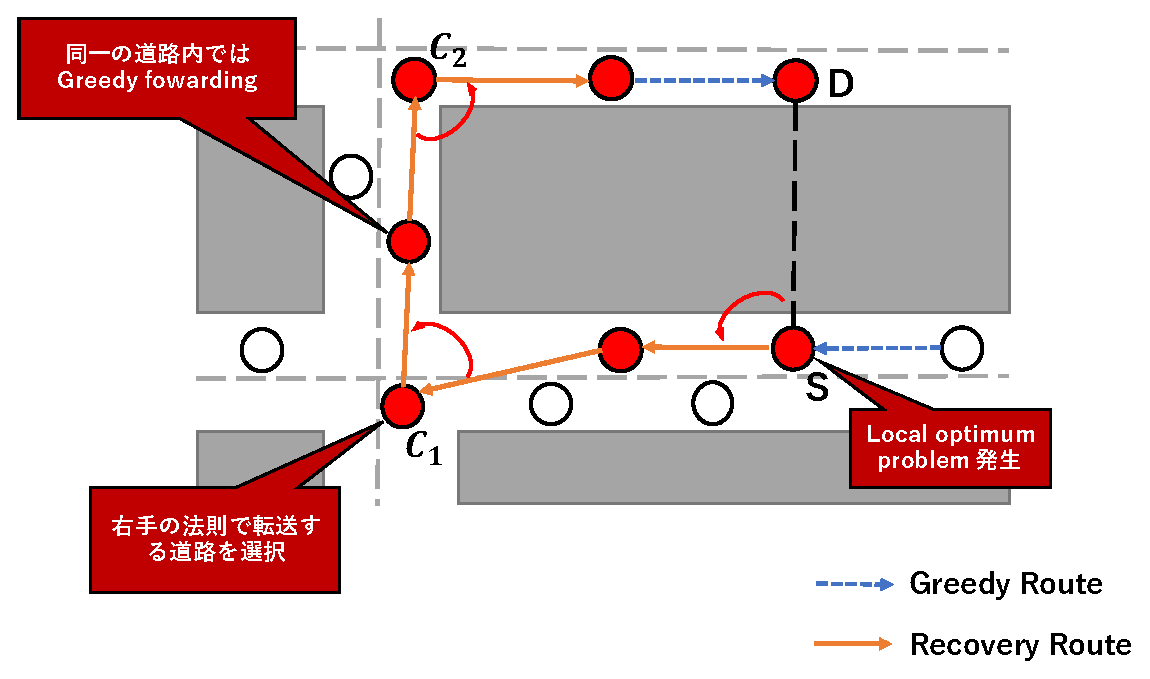
\includegraphics[width=130mm]{figures/GPCR.eps}
	\caption{GPCR}
	\label{fig:GPCR}
\end{figure}

Junction-Based Routing (JBR) \cite{JBR}のrecovery strategyでは, GPSRやGPCRのような右手の法則ではなく, 新たに最小角度法と呼ばれる手法を用いて中継ノードを選択する. JBRでは, 図\ref{fig:JBR}に示すように, 交差点ノードまでは従来の方式と同様にgreedy fowarding, 交差点ノードまでパケットが到達した場合, 交差点ノードは最小角度法に従って中継ノードを選択する. 図の例ではノードBが選択されている. 最小角度法の利点は, 右手の法則のようなループが起きないことである. 
しかし, JBRやGPCRのように交差点中心のrecovery strategyでは, 交差点ノードが存在しない場合アルゴリズムが機能しないという問題が発生する. また, JBRやGPCRなどの交差点中心のrecovery strategyを提案している既存研究の多くは, 建物によって電波が完全に遮断される仮定を基に, アルゴリズムが設計されている. これは現実的な仮定ではない. 
本研究ではこれらのrecovery strategyの問題に対処する新しいアルゴリズムを提案する. 

\begin{figure}[!ht]
	\centering
	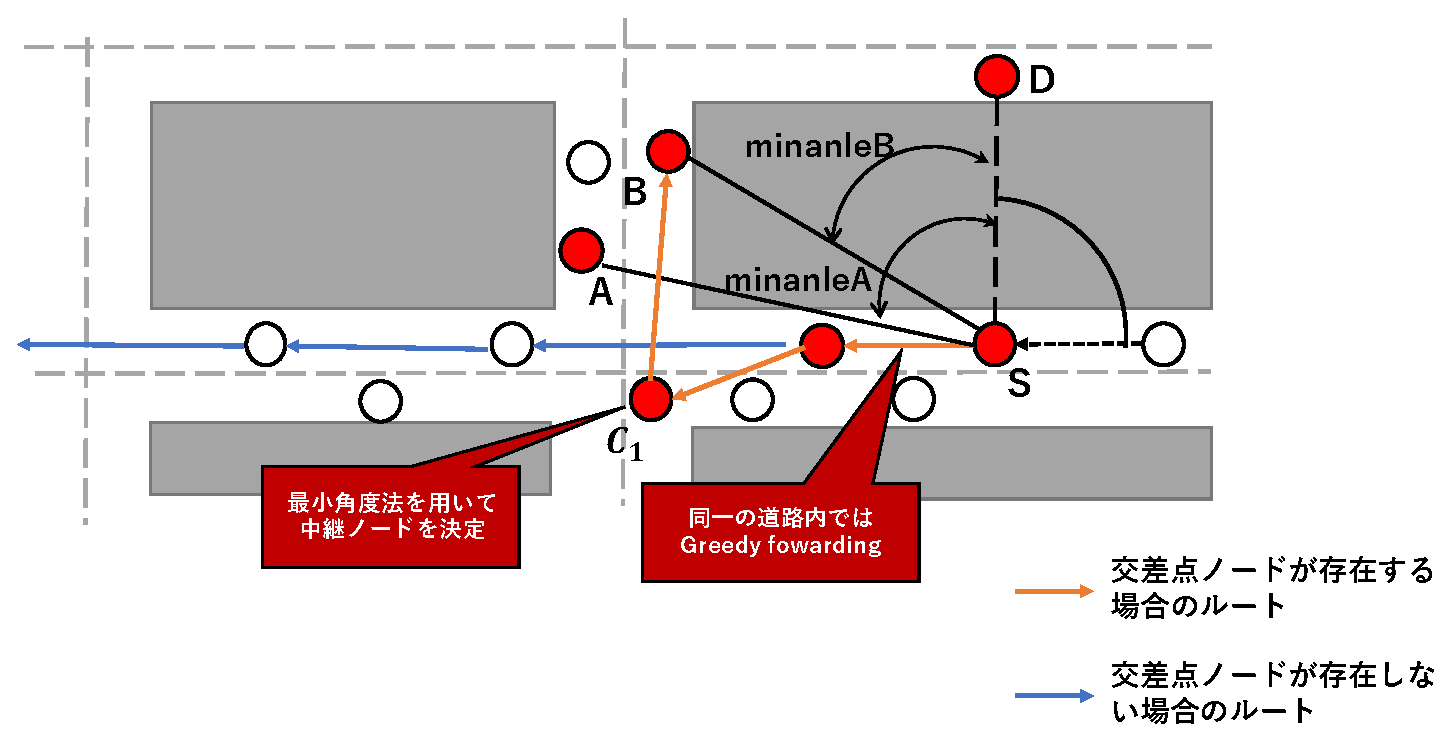
\includegraphics[width=140mm]{figures/JBR.eps}
	\caption{JBR}
	\label{fig:JBR}
\end{figure}



\chapter{LSGO}
\label{LSGO}
\section{概要}
LSGOはVANET用に設計されたopportunistic routingでは代表的なものの一つである.
LSGOでは, 各ノードは自ノードのIDと現在の位置情報で交際されるHelloパケットを定期的にブロードキャストする. これにより各ノードは隣接ノードの情報を得ることができる.
送信ノード(ソースノードまたは任意の$i$ホップ目の中継ノード)は, Helloパケットで取得した情報に基づいて, 中継候補ノードセット:RCSの選定とそれらに優先順位を割り当て, データパケットをブロードキャストする. 各送信ノードは次節以降で説明する, リンク品質と宛先までの距離の2つのメトリックに従って, RCSの優先順位を決定する. データパケットを受信した各ノードは, 自身のIDが含まれているかどうかを確認し, 含まれていない場合はパケットを破棄する. 含まれていた場合, 優先順位をチェックし, 次節で説明する優先度スケジューリングアルゴリズムに従ってパケットを再ブロードキャストするか否かを決定する.

\section{リンク品質の推定}
LSGOでは, 各ノードがHelloパケットを定期的にブロードキャストし, それを用いてリンク品質ETXを推定する. Helloパケットは, 自ノードのID, X座標, Y座標で構成されている. ETXを算出するために, 各ノードは近隣ノードから最初にHelloパケットを受信した時間$t_{0}$を記録する. そして, 現在時刻を$t$, ウィンドウサイズを$w$(second), Helloパケットの送信間隔を$\tau$とすると, 予想伝送確率$r(t)$はウィンドウサイズ$w$で場合分けされ, 式(\ref{trans-prediction})で算出される.

\begin{equation}
	\label{trans-prediction}
	r(t) =\begin{cases}count(t, t_{0}), & 0 < t - t_{0} < 1,  \\ \frac{count(t,t_{0})}{(t-t_{0}) / \tau}, & 1 \leq t - t_{0} \leq w\\
		\frac{count(t - w,t)}{w / \tau}, &  t - t_{0} \geq w\\
	\end{cases}
\end{equation}


ウィンドウサイズ$w$は, $r(t)$を算出する際に, 現在時刻$t$より以前に取得したHelloパケットの有効期間である. 例えば, 現在時刻$t$=10(s), ウィンドウサイズ$w$=5(s)とすると, 時刻5(s)より古いHelloパケットの情報は$r(t)$を算出する際には用いない. $(t,t_{0})$ / $\tau$は, ウィンドウサイズの間に受信されるべきHelloパケット数であり, $count(t,t_{0})$は$t$ ~ $t_{0}$の期間中に実際に受信されたHello パケットの数である. \par
各近隣ノードとのリンクの非対称性は考慮せず, 一方向の予想伝送確率$r(t)$のみを使用してETXを計算する. 一方向伝送確率が$r(t)$であると仮定すると, リンクETXは式(\ref{equ-intersection})で算出される.

\begin{equation}
	\label{equ-intersection}
	ETX = \frac{1}{  {r(t)}^{2}   } 
\end{equation}

\section{優先度スケジューリングアルゴリズム}

LSGOでは, タイマーベースの優先度スケジューリングアルゴリズムを使用する. このアルゴリズムでは, 最も優先度が高いノードが最初にパケットを送信する. ほかの候補ノードは, 優先順位の高いノードからのパケットを受信すると, 自身のパケットを破棄する. タイマーが期限切れになり, 自身より優先度の高いノードからのパケットを受信していない場合, 送信を開始する. LSGOは以下の式(\ref{pri})によって, ノード$i$の優先度が算出される.

\begin{equation}
	\label{pri}
	\frac{D_{sd} - D_{id}}{ETX_{i}^{2}} ,   D_{id} < D_{sd}
\end{equation}

$D_{sd}$は送信ノードから宛先ノードまでの距離, $D_{id}$は中継候補ノード$i$から宛先ノードまでの距離である.  $D_{id}$ < $D_{sd}$の条件を満たさない場合は, 優先度の計算を行わずにRCSから除外する.
式(\ref{pri})で算出された値が大きいほどノード$i$の優先順位が高くなる. 

\section{RCS選択アルゴリズム}
Opportunistic routingにおいてRCSに含まれるノード数が多い場合, バックアップリンクの数が多くなるためパケット到達率は向上するが, RCSに含まれるノード同士の協調(再ブロードキャストキャンセル)がされない確率が高まるというトレードオフが存在する.  
このためLSGOでは, 信頼性を確保しながら, 送信回数を減らすためにRCSに含まれるノード数を最適化するアルゴリズムが提案されている.  
式(\ref{pri})を用いて各隣接ノードの優先順位を$p$ = 1,2..$N$(1が最も優先順位が高い)とすると, $N$は次の条件を満たす必要があり, RCSに含まれるノードはは1~$N$に制限される. 

\begin{equation}
	\label{Min-Probability}
	1 - \prod_{p=1}^N (1 - r_{p}(t))\geq R
\end{equation}

式(\ref{Min-Probability})における$r_{p}(t)$ (1$ \leqq $p$ \leqq $N)は, 送信ノードが保持する隣接ノード(優先順位$p$)に対する予想伝送確率である. 
式(\ref{Min-Probability})の左辺は送信ノードからのパケットを候補ノード1~$N$のいずれかのノードが受信すると予想される確率であり, 右辺$R$はその確率の閾値である. $R$が大きいほど, RCSに含まれるノード数が増加し, 小さくなるほどRCSに含まれるノード数が減少する. 車両密度が小さい場合や送信ノードと各隣接ノード間の予想伝送確率が低い場合, 式(\ref{Min-Probability})満たすことができない場合がある. その場合, $D{id}$ \verb|<| $D_{sd}$の条件を満たすすべての隣接ノードがRCSとして選択される. また, 送信ノードと各隣接ノードとの予想伝送確率が高い場合, 候補ノード数$N$は小さくなるため, 信頼性を確保しながら, 最低限の候補ノード数を選択することができる. 


\section{シャドウイングとRCS数の影響}
本節では, シャドウイングによる電波減衰が起きやすい都市環境において, RCSに含まれるノード数がどのように通信性能に影響を与えるのか, LSGOのRCS選択アルゴリズムは有効なのかを調査する.
また, シャドウイングによる電波減衰が起こる場合と起こらない場合とでのLSGOの通信性能に与える影響を調査する.

\subsection{シミュレーション設定}
シミュレーションパラメータを表\ref{tab:parameter}, シミュレーションシナリオを図\ref{fig:Scnario}に示す. シミュレーションシナリオは交通流シミュレータのSUMO\cite{27}を使用して作成した. シミュレーション開始時に, ランダムな送信ノードと宛先ノードがそれぞれ10台ずつ割り当てられ, 通信を開始する. 各交差点には信号機を配置し, 図の灰色の領域に建物を配置した. 
NS-3の電波伝搬モデルとしてシャドウイングモデルであるObstacle shadowing model\cite{20}を使用した. シャドウイングによる伝搬損失$L_{s,o}$は各壁による損失と建物の貫通距離(m)に基づいて式(\ref{shadowing})で算出される.

\begin{equation}
	\label{shadowing}
	L_{s,o} = \alpha n  + \beta d_0
\end{equation}

シャドウイングモデルには2つのパラメータが存在する. $\alpha$は壁あたりの減衰(db), $\beta$は建物の貫通距離あたりの減衰(db)である. また, $n$は貫通した建物の壁の数であり, $d_{o}$は建物の貫通距離(m)である.
本シミュレーションでは, $\alpha$= 10 dB and $\beta$= 0.4 dB で評価を行った. 

\begin{figure}[!ht]
	\centering
	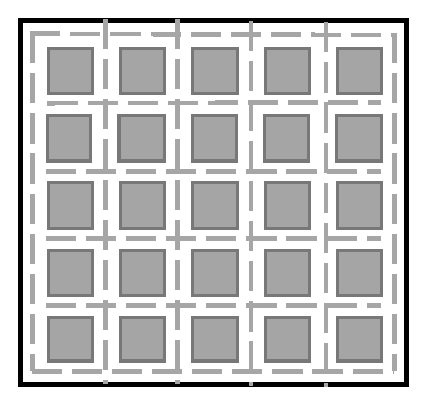
\includegraphics[width=70mm]{figures/Scenario.eps}
	\caption{シミュレーションシナリオ}
	\label{fig:Scenario}
\end{figure}

\begin{table}[!ht]
	\begin{center}
		\caption{シミュレーションパラメータ}
		\label{tab:parameter}
		\begin{tabular}{|l|l|lll}
			\cline{1-2}
			Network Simulator    & NS-3 (v3.30) &  &  &  \\ \cline{1-2}
			Traffic Simulator    & NS-3 (v3.30) &  &  &  \\ \cline{1-2}
			Simulation area    & 1000m × 1000m   &  &  &  \\ \cline{1-2}
			Mobility model     & Random mobility &  &  &  \\ \cline{1-2}
			Transmission range & 250m            &  &  &  \\ \cline{1-2}
			Number of vehicles & 200, 300, 400      &  &  &  \\ \cline{1-2}
			Radio propagation model    & obstacle shadowing model\cite{20}&  &  &  \\ \cline{1-2}
			MAC Layer     & 802.11p &  &  &  \\ \cline{1-2}
			Packet Size & 512 byte       &  &  &  \\ \cline{1-2}
			Simulation Time & 30 s      &  &  &  \\ \cline{1-2}
			hello interval & 1 s      &  &  &  \\ \cline{1-2}
			Window size w  & 10 s      &  &  &  \\ \cline{1-2}
			%Number of relay candidate nodes  & 5       &  &  \\ \cline{1-2}
			shadowing parameter $\alpha$  & 10db      &  &  &  \\ \cline{1-2}
			shadowing parameter $\beta$    & 0.4db &  &  \\ \cline{1-2}
		\end{tabular}
	\end{center}
\end{table}

\subsection{評価項目}
本シミュレーションでは, LSGOの通信性能を評価するためパケット到達率(PDR), エンドツーエンド遅延(Delay), オーバーヘッド(Overhead)の3つの評価項目で評価した. PDR, Delay, Overheadの算出式をそれぞれ式\ref{PDR}, \ref{delay}, \ref{overhead}に示す.

\begin{equation}
	\label{PDR}
	PDR = \frac{D_{recv}}{  S_{sent}  } \times 100
\end{equation}

ここで, PDRはソースノード(データパケットを一番初めに生成したノード)から宛先ノードに送信されるパケットの到達率を表す. $S_{sent}$はソースノードが送信した合計パケット数を表し, $D_{recv}$は宛先ノードが受信した合計パケット数を表す.

\begin{equation}
	\label{delay}
	Delay = \frac{\sum_{i=1}^{N}ED_i}{N}
\end{equation}

ここでエンドツーエンド遅延(秒)は, ソースノードがパケットを送信してから宛先ノードに到達するまでにかかる平均時間を表す. $ED_i$は, 宛先ノードが正常に受信したパケット$i$(1$ \leqq $i$ \leqq $N)が, ソースノードの送信から宛先ノードに到達するまでにかかる時間を表す. 
$N$は宛先ノードが正常に受信したパケット数を表す.

\begin{equation}
	\label{overhead}
	Overhead = \frac{N_{sent}}{  D_{recv}  }
\end{equation}

ここでオーバーヘッドは, 1データパケットを宛先ノードに届けるためにどれだけのパケット数を費やしたかを表す. $N_{sent}$はネットワーク全体における各ノードが送信した合計パケット数を表す.

\subsection{RCS数の影響}
本シミュレーションでは, RCSに含まれるノード数が通信性能にどのように影響するのかを評価した.
シャドウイングパラメータ$\aleph$ = 10, $\beta$ = 0.4, ノード数は400に設定した.
図\ref{fig:RCS-PDR}, \ref{fig:RCS-delay}, \ref{fig:RCS-overhead}は, RCS数を変化させたときのパケット到達率, エンドツーエンド遅延, オーバーヘッドを示している. RCS\_LSGOは, RSC数をLSGOのアルゴリズムに従って決定した場合の取得データを示している. 今回のシミュレーションでは, 式\ref{Min-Probability}の閾値$R$は, RCS数が最も多くなる1.0に設定した. RCS\_1~5はRCS数を1~5個に設定した時の取得データを示している. また, RCS\_1~5の時のRCS数は最大値であり, 各送信ノードより宛先ノードに近いノードが設定したRCS数より少ない場合, 隣接するすべてのノードがRCSに含まれる.
\par
\vspace{5mm}
\noindent
\textbf{パケット到達率(PDR)}
\vspace{5mm}


図が示す通り, RCS数が増加するほどパケット到達率が向上している. これはRCS数が多いほど, RCSに含まれるノードのいずれかにパケットが到達する確率が上昇するからである. また, 本シミュレーションシナリオとobstacle shadowing modelを用いて評価した場合, LSGOのRCS選択アルゴリズムの性能が低いことがわかる. LSGOのRCS選択アルゴリズムは予想伝送確率を使用して設計されており, 予想伝送確率はHelloパケットの受信履歴から計算される. しかし, 実際のHelloパケットはデータパケットよりもデータサイズが小さいため, データパケットより高確率で受信される. これがこのアルゴリズムの性能低下の原因だと推測される.

\begin{figure}[!ht]
	\centering
	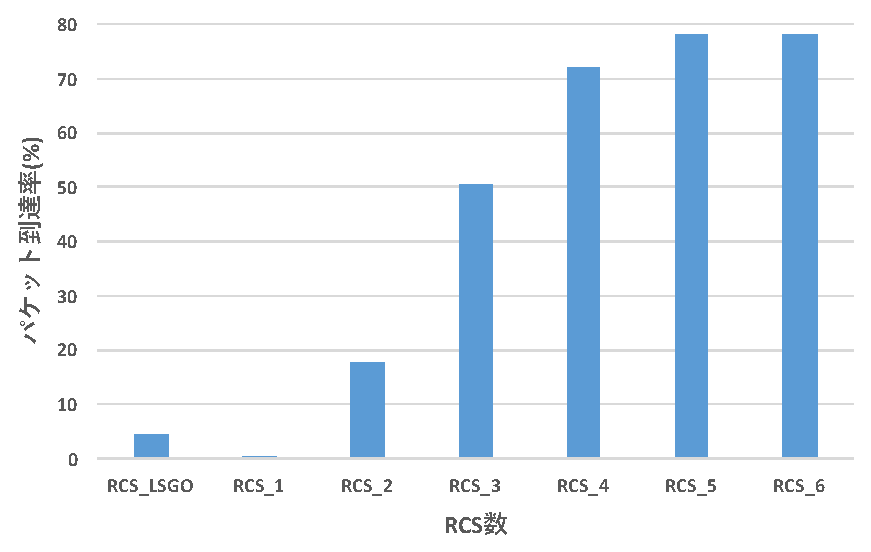
\includegraphics[width=110mm]{figures/RCS_PDR.eps}
	\caption{RCS数の変化にともなうPDR}
	\label{fig:RCS-PDR}
\end{figure}

\par
\vspace{5mm}
\noindent
\textbf{エンドツーエンド遅延}
\vspace{5mm}

図が示す通り, RCS数が増加するほど, 遅延は増加している. これは2通りの理由が推測される. 1つ目は, RCS数が少ない場合, ソースノードと宛先ノードの距離が近い場合のみ宛先ノードが正常にパケットを受信したからである. 図\ref{fig:RCS-hop}に, 送信ノードから宛先ノードまで正常に到達したパケットの平均ホップ数を示す. RCS数が少ない場合, ホップ数が減少していることがわかる. これはRCS数が少ない時には, 送信ノードと宛先ノードの距離が近い場合に限り, 正常にパケットが到達したことを示している.
2つ目は, RCS数が多いほど, 優先順位が低い中継候補ノードのみパケットを受信した場合, 優先順位の低いノードほど待ち時間(中継タイマー)が長いからである.




\begin{figure}[!ht]
	\centering
	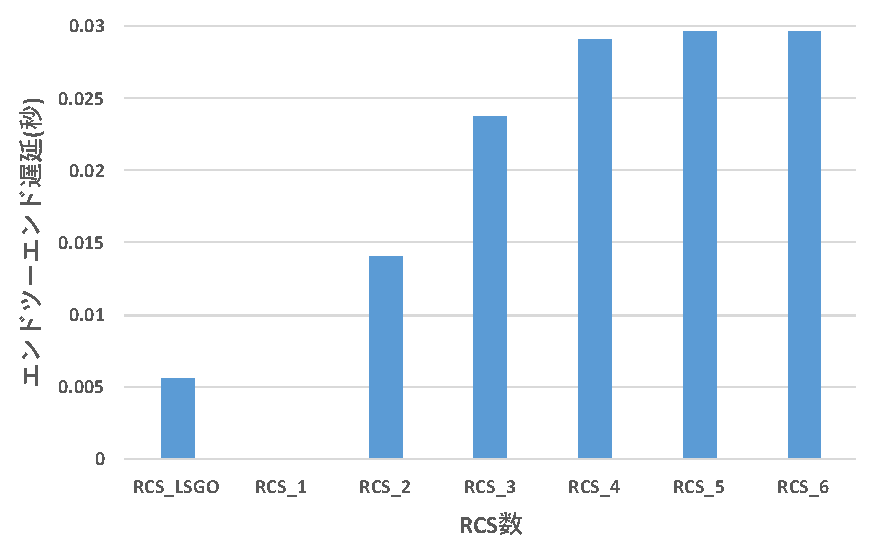
\includegraphics[width=110mm]{figures/RCS_Delay.eps}
	\caption{RCS数の変化にともなうエンドツーエンド遅延}
	\label{fig:RCS-delay}
\end{figure}

\par
\vspace{5mm}
\noindent
\textbf{オーバーヘッド}
\vspace{5mm}

図が示す通り, RCS数が増加するほど, オーバーヘッドが減少している. これはRCSが増加するほど, ネットワーク全体における各ノードが送信した合計パケット数は増加しているが, 宛先ノードが正常に受信したパケット数も増加したためである. また, ホップ数が著しいRCS数1を除き, RCS数が増加するほどオーバーヘッドが減少しているが, 5から6にかけて少し増加している. これは, 5から6にかけて宛先が正常に受信したパケット数に差がないのに対して, ネットワーク全体における各ノードが送信した合計パケット数が増加しているからである. したがって, 本シミュレーションではRCS数5の場合が最も効率的である. 

\begin{figure}[!ht]
	\centering
	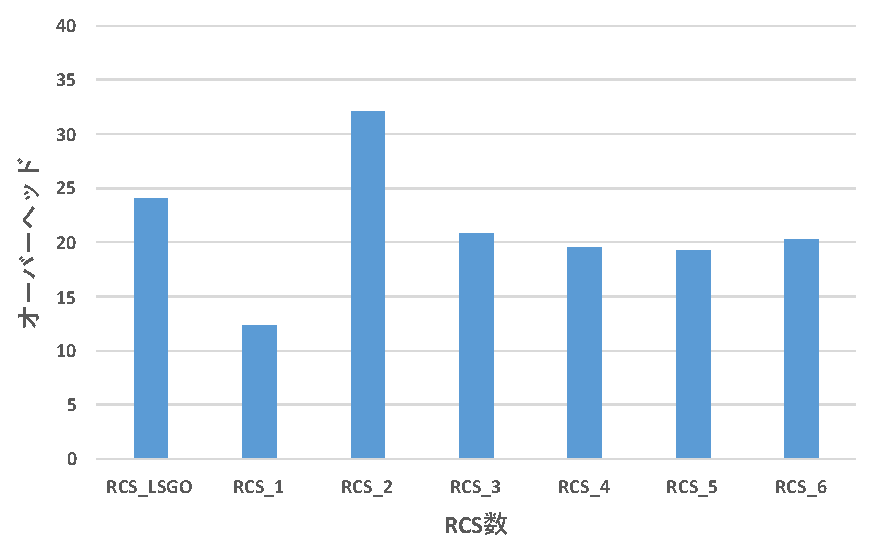
\includegraphics[width=110mm]{figures/RCS_Overhead.eps}
	\caption{RCS数の変化にともなうオーバーヘッド}
	\label{fig:RCS-overhead}
\end{figure}

\begin{figure}[!ht]
	\centering
	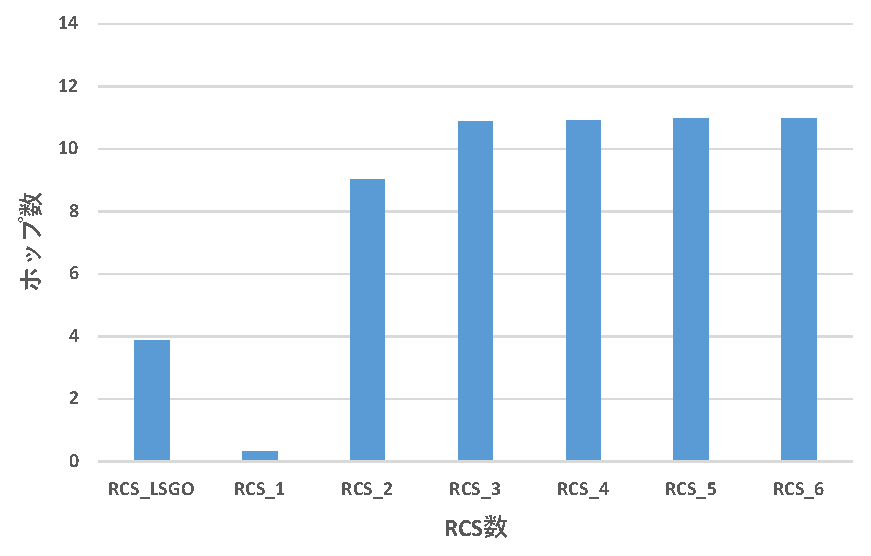
\includegraphics[width=110mm]{figures/RCS_Hop.eps}
	\caption{RCS数の変化にともなうホップ数}
	\label{fig:RCS-hop}
\end{figure}

\subsection{シャドウイングの影響}
本シミュレーションでは, 建物のシャドウイングによる電波の減衰が起こる場合のLSGOの通信性能に与える影響を評価した.
またRCS数は5に設定した.

\par
\vspace{5mm}
\noindent
\textbf{パケット到達率}
\vspace{5mm}

図\ref{fig:LSGO-PDR}は, ネットワークシミュレーションでシャドウイングの影響を考慮した場合としない場合とでの, パケット到達率を示している.
シミュレーションでシャドウイングを考慮した場合, 全てのノード数においてパケット到達率が減少している. これは, シャドウイングによる電波減衰が原因だと推測される.



\begin{figure}[!ht]
	\centering
	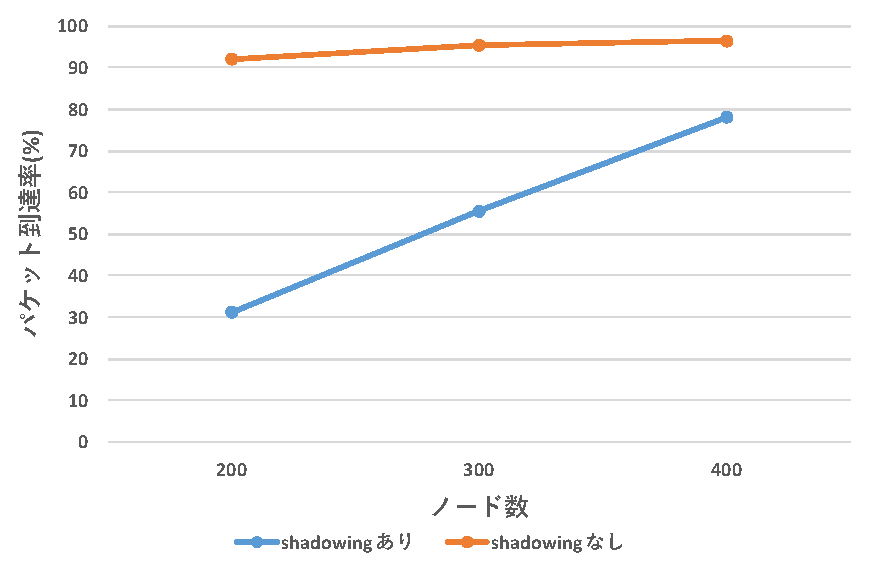
\includegraphics[width=110mm]{figures/LSGO_PDR.eps}
	\caption{パケット到達率 シャドウイングの有無}
	\label{fig:LSGO-PDR}
\end{figure}

\par
\vspace{5mm}
\noindent
\textbf{エンドツーエンド遅延}
\vspace{5mm}

図\ref{fig:LSGO-delay}は, はネットワークシミュレータでシャドウイングの影響を考慮する場合としない場合とでのエンドツーエンド遅延(秒)を
示している. シミュレーションでシャドウイングを考慮した場合, 全てのノード数においてエンドツーエンド遅延が増加している. これはシャドウイングによる電波減衰が起こり, 建物を通過するパケットが届きにくくなることで,  ソースノードと宛先ノードを直線的に結ぶような経路が形成することが難しくなったことが原因だと考えられる.

\begin{figure}[!ht]
	\centering
	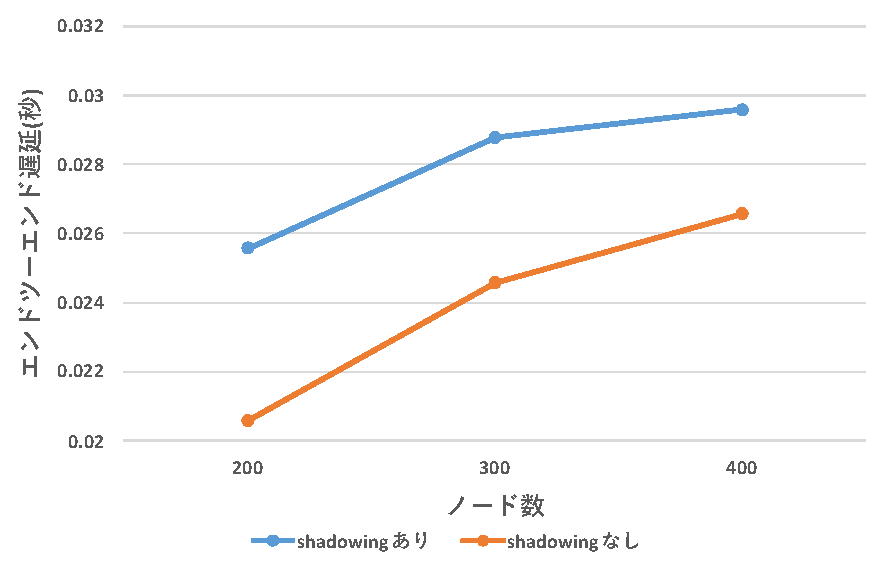
\includegraphics[width=110mm]{figures/LSGO_delay.eps}
	\caption{エンドツーエンド遅延 シャドウイングの有無}
	\label{fig:LSGO-delay}
\end{figure}


\par
\vspace{5mm}
\noindent
\textbf{オーバーヘッド}
\vspace{5mm}

図\ref{fig:LSGO-overhead}は, ネットワークシミュレータでシャドウイングの影響を考慮した場合としない場合とでのオーバーヘッドを示している.
シミュレーションでシャドウイングを考慮した場合, すべてのノード数においてオーバーヘッドが増加している. これは2通りの理由が推測される.
1つ目は, シャドウイングによる電波減衰が起こり, 建物を通過するパケットが届きにくくなることで,  ソースノードと宛先ノードを直線的に結ぶような経路が形成することが難しくなったため, ホップ数が増加したと推測される. 
2つ目は, opportunistic routingでの送信ノードから指定されたRCSに指定されたノード同士が自分より優先度の高いノードからのパケットを建物による電波減衰によって, 受け取れない確率が増加し, 再転送がキャンセルされていないことが原因だと推測される.


\begin{figure}[!ht]
	\centering
	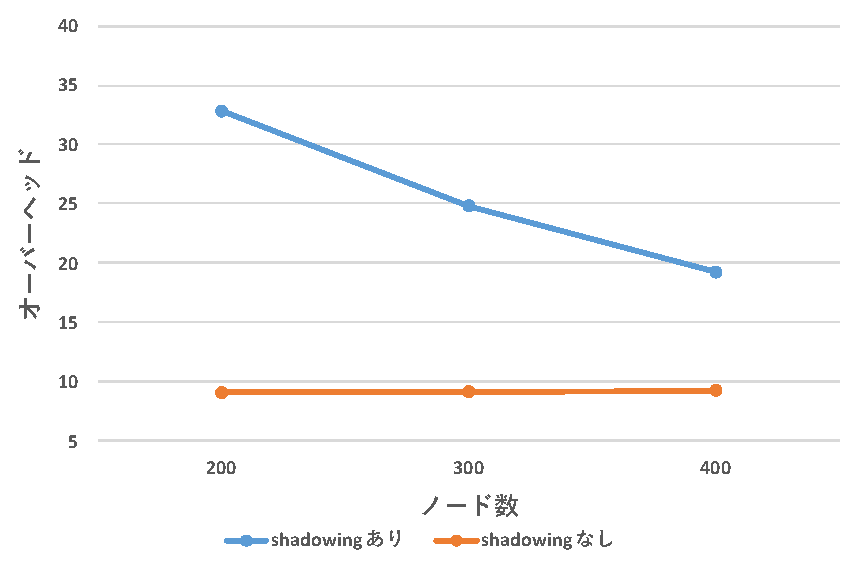
\includegraphics[width=110mm]{figures/LSGO_overhead.eps}
	\caption{オーバーヘッド シャドウイングの有無}
	\label{fig:LSGO-overhead}
\end{figure}


\subsection{LSGOの問題点}
本節では, LSGOの中継戦略の問題点について考察する. LSGOでは, 中継候補ノードの優先順位をあて先ノードまでの近さとリンク品質を基に決定する. 問題のあるシチュエーションの一例を図\ref{fig:LSGO-problem}に示す. 

\begin{figure}[!ht]
	\centering
	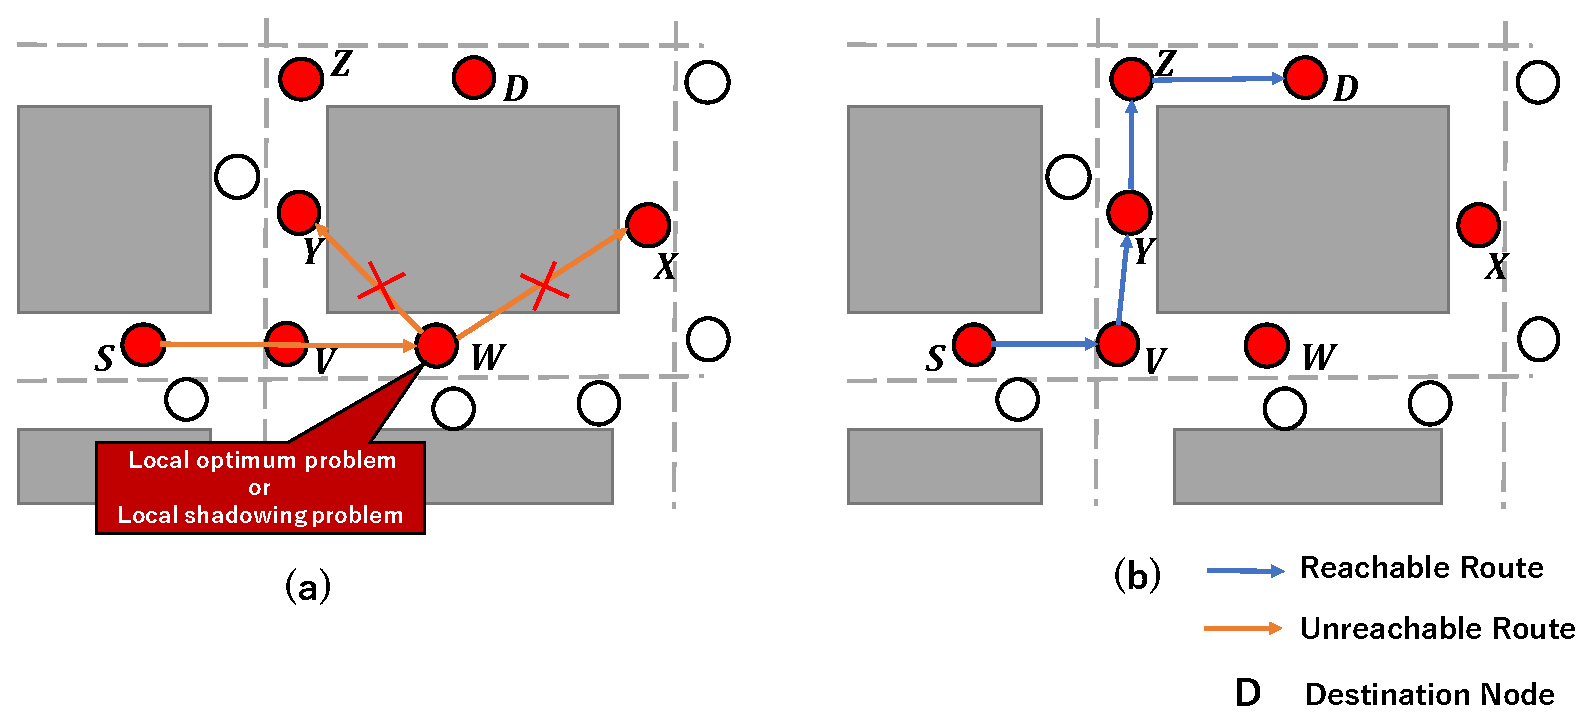
\includegraphics[width=160mm]{figures/LSGO_problem.eps}
	\caption{中継戦略の問題点}
	\label{fig:LSGO-problem}
\end{figure}

図(a)のように送信ノード$S$が, ノード$W$を最も優先度の高い中継ノードとして選択した場合を考える. この場合, ノード$W$に続く中継ノード(ノード$W$より宛先に近いノードを選択)は, シャドウイングによりリンク品質が良くないノード$X$と$Y$のみとなる. この問題をLocal shadowing problemと呼ぶ. また, シャドウイングの強度が強い場合, $X$と$Y$のリンクが完全に遮断されている場合が考えられる. この場合, \ref{local_optimum_problem}節で紹介したLocal optimum problemが発生する. これらのことから, LSGOの中継戦略は, Local shadowing problemやLocal optimum problemに陥る可能性が高いことがわかる. この問題は, 図(b)に示すように, ノード$V$のような交差点ノードを中継ノードとして選択することで回避することができる. 





\chapter{車両位置とリンク状態を考慮した地理的opportunistic routing}
\section{概要}
本研究では, 以下の3つを提案する. \par
\textbf{1. シャドウイングを考慮したopportunistic routing(SIGO)} \par
\textbf{2. シャドウイングを考慮したrecovery strategy(ORS)} \par
\textbf{3. 1のoppotrunistic routingを基に拡張したgeocast routing} \par

1ではLSGOの問題点を解決するopportunistic routingを提案する. 性能評価では, LSGOとの比較を行った. 2では, 既存recovery strategyの問題を解決するopportunistic recovery strategy提案する. 提案するrecovery strategyと比較手法としてJBRをSIGOのrecovery strategyとして加え比較を行った.
3では, SIGOとLSGOをそれぞれgeocast routingに拡張し, それぞれの比較を行った.

\subsection{SIGO: Shadowing-based Intersection Geographic Opportunistic Routing}

本研究では, shadowing-based intersection geographic opportunistic routing(SIGO)という, シャドウイングを考慮したopportunistic routingを提案する. SIGOでは, 中継ノードの優先度を決定するメトリックとして, 宛先ノードまでの距離, リンク品質に加え, 交差点ノードを優先する指標である$IRI$(intersection relay index)を用いる. 最初の2つのメトリックは, \ref{LSGO}章で紹介したLSGOと同様の方法で算出する.

\subsection{ORS: Opportunistic Recovery Strategy}

\subsection{Geocast routingへの拡張}






\addcontentsline{toc}{chapter}{謝辞}
\chapter*{謝辞}
\sloppy
本論文では筆者が立命館大学情報理工学部情報コミュニケーション学科におい
て行なった「VANETを用いた速度超過車両検出のためのブロードキャスト制御法」の成果をまとめたものである.

本研究を遂行するにあたり,全過程を通じて懇切丁寧なる御指導,御鞭撻を賜わっ
た,立命館大学情報理工学部野口~拓教授に深甚なる感謝の意を表す.

立命館大学情報理工学部において,御指導,御教授を賜わった立命館大学情報理工学部Alberto Gallegos Ramonet特任助教, 前田~忠彦教授, 山本~寛准教授, 西村~俊和准教授, 瀧本~栄二助教を始め,各教員の方々に衷心より御礼申し上げる.

%本研究を遂行するにあたり,終始一貫して直接御指導戴いたネットワークシステム研究室の野口~拓講師に深甚なる感謝の意を表す.

ネットワークシステム研究室の諸兄には,日頃より多くの御助言,御協力戴き,種々の面でお世話になった.ここに深謝申し上げる.

ここに記して,以上の方々に深甚なる感謝の意を捧げる.

\addcontentsline{toc}{chapter}{参考文献}

%\newpage

\bibliographystyle{IEEEtran}
\bibliography{shuto}


\end{document}
